\chapter{User Studies}\label{chapter:userstudy}

A total of two user studies were conducted. The user studies were held in the GamesLab on TUM Campus Garching. The participants were compensated with beverages and/or sweets. Beforehand the participants were informed about the aim of the study as well as their specific objectives. 

\begin{figure}[h]
\centering
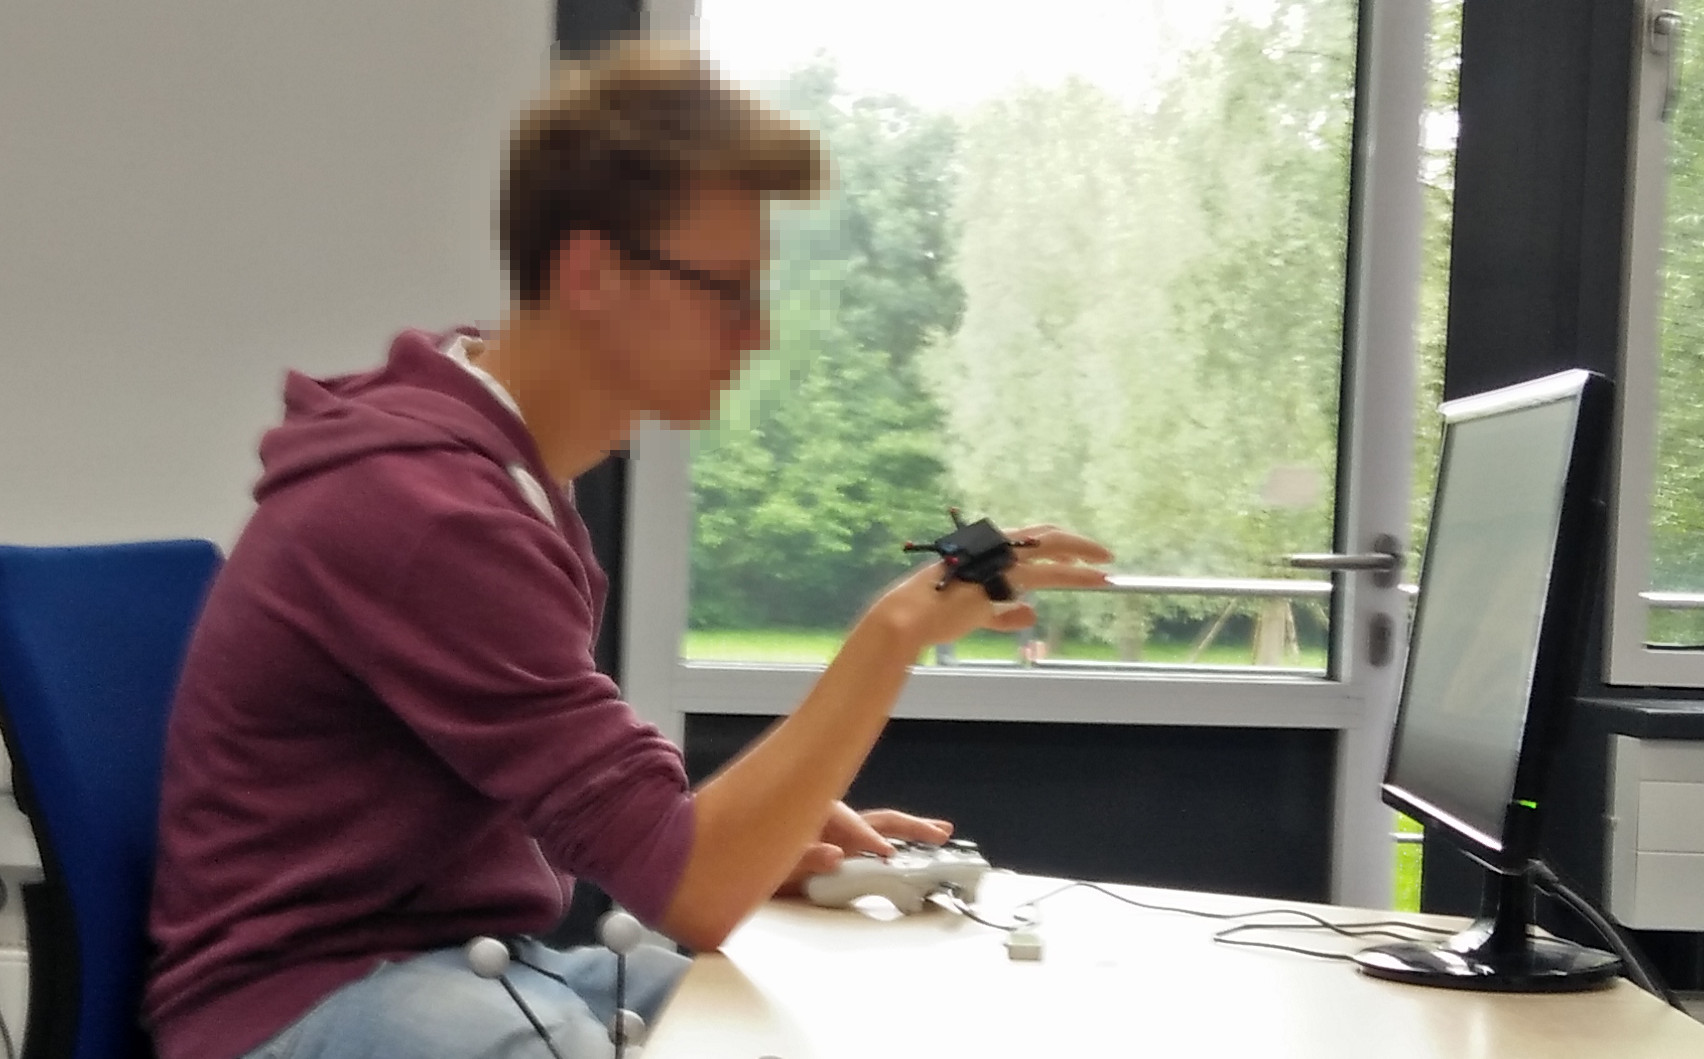
\includegraphics[width=\textwidth]{baschde}
\caption{A Participant performing the Target Shooting Test.}
\label{fig:baschde}
\end{figure}

\section{Pilot User Study}

The first user study had 12 participants, aged between 19 and 40 consisting of 2 women and 10 men. None of the subjects were closely familiar with the research topic. The participants were scheduled individually for 30 minute slots, the the average user study took 20 minutes.
The participants had to carry out 5 hand posture comfort evaluations and 4 rounds of target shooting and line tracing as described above. 

For target shooting and line tracing the participants were told to maintain a balance between speed and accuracy. The idea behind this was to measure performance and precision in the form of total task time and average target accuracy. 

\section{Early Analysis and its Consequences}

Early analysis of the resulting data revealed, that computed naive metric values did actually seem to correlate with the user ratings for the hand posture evaluation task. However, when comparing the computed metric values or the user ratings to precision or time taken in the target shooting and line tracing task, only noise was visible. 
For this we suspected to have following reason: Already during the user study it was noticeable that different people had different understandings of "a balance between accuracy and speed". Thus some people were taking their time to aim at the exact center of the target while others just did everything as quickly as possible.
In addition to that, the amount of data collected was nowhere near to get be able to create the improved metric.

Hence some modifications to the test environment had to be made. In order to work off more participants the time slots were reduced to 20 minutes. The target shooting test was modified, the number of targets was reduced from 18 to 12. In order to solve the "accuracy-time" problem the targets were made smaller so that they are harder to hit and the participants were told to only focus on speed. The idea behind this is that the smaller target size will affect the accuracy needed to hit them as described by Short et al. \cite{short1999precision}. Hence, if a hand posture influences the accuracy in a pointing task, the participant will take longer to aim at the target. This way both performance and precision are represented by the total task time. 
For the line tracing task, no such optimization was possible. Since participants had struggled with this task to begin with, it was simply discarded.
In order to collect enough data for the improvement of the metric, the number of hand posture evaluations was increased from 5 to 15.

\section{Second User Study}

15 people participated in the second user study, thereof 5 women and 10 men aged between 19 and 25. Again none of the subjects were closely familiar with the research topic.
Due to the ART hand tracker breaking down during the 9th user study, only 35 samples of the target shooting test could be collected. To fill the resulting time gap, the remaining participants were asked to do 20 hand posture comfort evaluations instead.
In total 250 data sets for hand posture evaluation were collected.